\chapter{Experimental Testing}
\label{chap:Experimental Testing}

\section{Virtual Spring-damper Tests} 
\label{sec:Virtual Spring-damper Tests}
$r_0 = 0.3\ m$\\
$r_{offset} = r - r_0 = 0.13\ m$

\subsection{Full-leg Spring Damper}

\begin{figure}
\centering
\includegraphics[width=1\textwidth]{images/experiments/spring-damper-tests2.eps} 
\caption{Full-leg spring damper testing for radial offset.}
\label{fig:spring-damper-tests}
\end{figure}

\begin{figure}
\centering
\includegraphics[width=1\textwidth]{images/experiments/full-leg-spring-damper-control-output.eps} 
\caption{Full-leg spring damper motor control.}
\label{fig:full-leg-spring-damper-motor-control}
\end{figure}

\subsection{Joint Spring Damper}

Scaling factor of 0.01...
\begin{figure}
\centering
\includegraphics[width=1\textwidth]{images/experiments/joint-spring-damper-tests.eps} 
\caption{Joint spring damper testing for radial offset.}
\label{fig:joint-spring-damper-tests}
\end{figure}

\begin{figure}
\centering
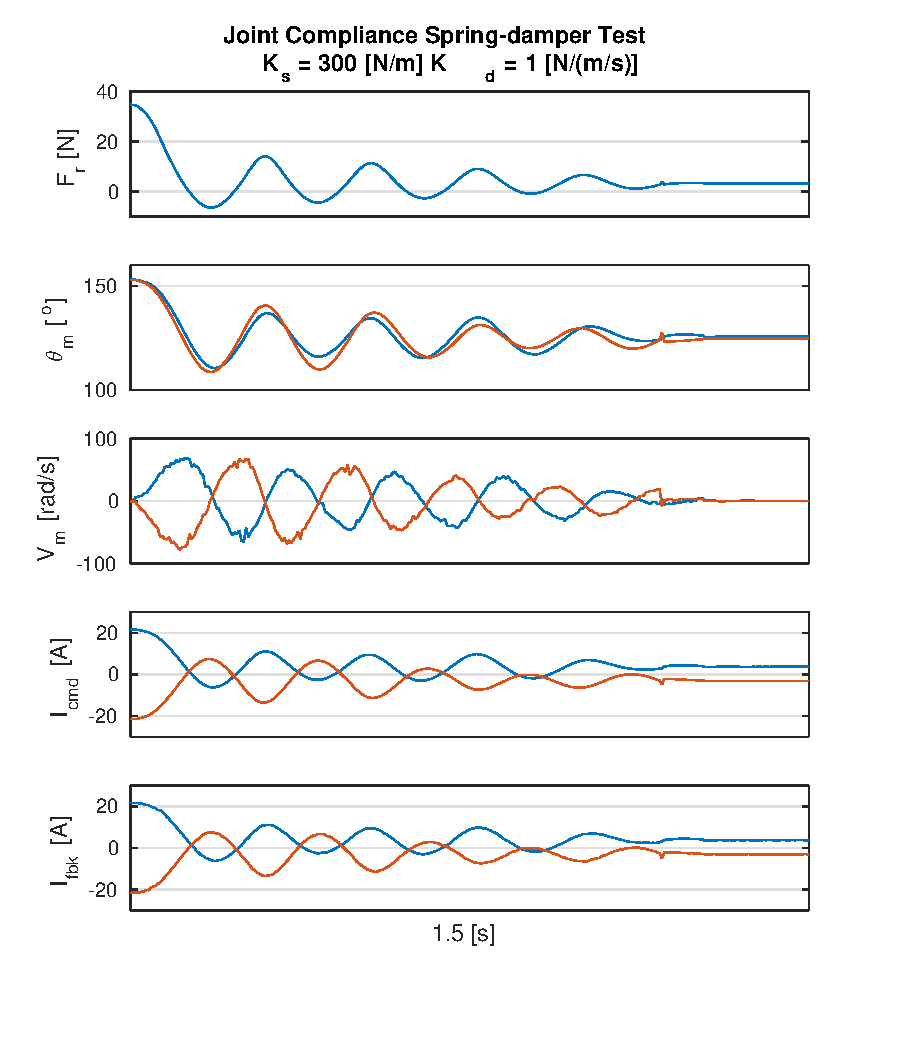
\includegraphics[width=1\textwidth]{images/experiments/joint-spring-damper-control-output.eps} 
\caption{Joint spring damper motor control.}
\label{fig:joint-spring-damper-motor-control}
\end{figure}

\subsection{Experimental Limitations}

\subsection{Data Analysis}

\section{Drop Tests}

A theoretical value for the spring constant $K_s$, with $K_d = 5 N/(m/s)$, for radial spring-damping upon impact was determined in \cref{sec:Leg Spring-damper Model} using conservation of energy and an ideal dynamic response. The calculated spring constant of $632.8\ N/m$ was used as a starting point for testing and the damping was varied from $0\ N/(m/s)$ to $5\ N/(m/s)$ to confirm the values derived.

\begin{figure}
\centering
\includegraphics[width=1\textwidth]{images/experiments/drop-test-force-plots.eps} 
\caption{Leg spring damper drop testing.}
\label{fig:drop-tests}
\end{figure}

\subsection{Experimental Limitations}

\subsection{Data Analysis}

\section{Jump Tests}

A summary of the jump phases and experimental setup can be seen in \cref{fig:jump-phases-experiment}. The radial foot forces experienced at each jump phase are included as well as the radial and rotational spring-damper constants. The development of this experiment will be expanded upon in more detail.

\begin{figure}
\centering
\includegraphics[clip, trim = 2.5cm 2cm 4cm 2cm, width=1\textwidth]{images/experiments/jump/jump-phases.pdf} 
\caption{Jump phases and experimental setup.}
\label{fig:jump-phases-experiment}
\end{figure}

\subsection{Configuration of Jump Phase Parameters}

Spring-damper mass motion of the leg model was theoretically developed in \cref{sec:Spring-damper Mass Motion}. Ideal spring-damper constants for flight, impact and launch were developed using conservation of energy relationships and spring-damper dynamic equations. 

The table of spring-damper constants and other configuration parameters, \cref{tbl:Leg launch virtual model configuration}, was found for ideal jump phase dynamics relating to the spring constants in \cref{fig:Leg spring-damper virtual model}. 

Parameters were derived both experimentally and theoretically. The theoretical (orange), drop test experimental (blue), and spring-damper test experimental (red) configuration parameters were highlighted appropriately.

\begin{table}[]
\centering
\begin{tabular}{llllll}
\textbf{Phase}       & \textbf{$K_{s1}\ [Nm]$}                 & \textbf{$K_{d1}\ [N/(m/s)]$}       & \textbf{$K_{s2}\ [N/m]$}     & \textbf{$K_{d2}\ [N/(m/s)]$} & \textbf{$r\ [m]$}                    \\
Stance               & 632.8                                   & \cellcolor[HTML]{00D2CB}15         & \cellcolor[HTML]{00D2CB}400 & \cellcolor[HTML]{00D2CB}5    & 0.25                                 \\
Decompression launch & \cellcolor[HTML]{FFC702}\textbf{1726.6} & \cellcolor[HTML]{FFC702}\textbf{0} & \cellcolor[HTML]{00D2CB}400 & \cellcolor[HTML]{00D2CB}5    & \cellcolor[HTML]{FFC702}\textbf{0.4} \\
Recovery             & \cellcolor[HTML]{FD6864}632.8           & \cellcolor[HTML]{00D2CB}15         & \cellcolor[HTML]{00D2CB}400 & \cellcolor[HTML]{00D2CB}5    & \cellcolor[HTML]{FD6864}0.3          \\
Compliant landing    & \cellcolor[HTML]{FFC702}\textbf{632.8}  & \cellcolor[HTML]{00D2CB}15         & \cellcolor[HTML]{00D2CB}400 & \cellcolor[HTML]{00D2CB}5    & \cellcolor[HTML]{FFC702}\textbf{0.3}
\end{tabular}
\caption{Leg launch virtual model configuration.}
\label{tbl:Leg launch virtual model configuration}
\end{table}

\subsection{Control Finite State Machine and Triggering}

\Cref{listing:Jump control condition loop} in \cref{app:Jump Experiment} shows the code implementation of a finite state machine that determines which spring-damper parameters are used in which phase of jumping. 

Using \textit{if statements} various conditions were tested to determine the phase of jumping.

Foot trigger techniques tried. Distance sensor too much noise...

\subsection{Testing Platform Setup}

\cref{subsec:Testing Platform}

\subsection{Video Data Extraction}

\cref{app:Jump Experiment}

\subsection{Experimental Limitations}

Current cut-out - refer to appendix \cref{app:Jump Experiment} \cref{fig:Motor driver over-current cut-out}

\subsection{Data Analysis}

\begin{figure}
\centering
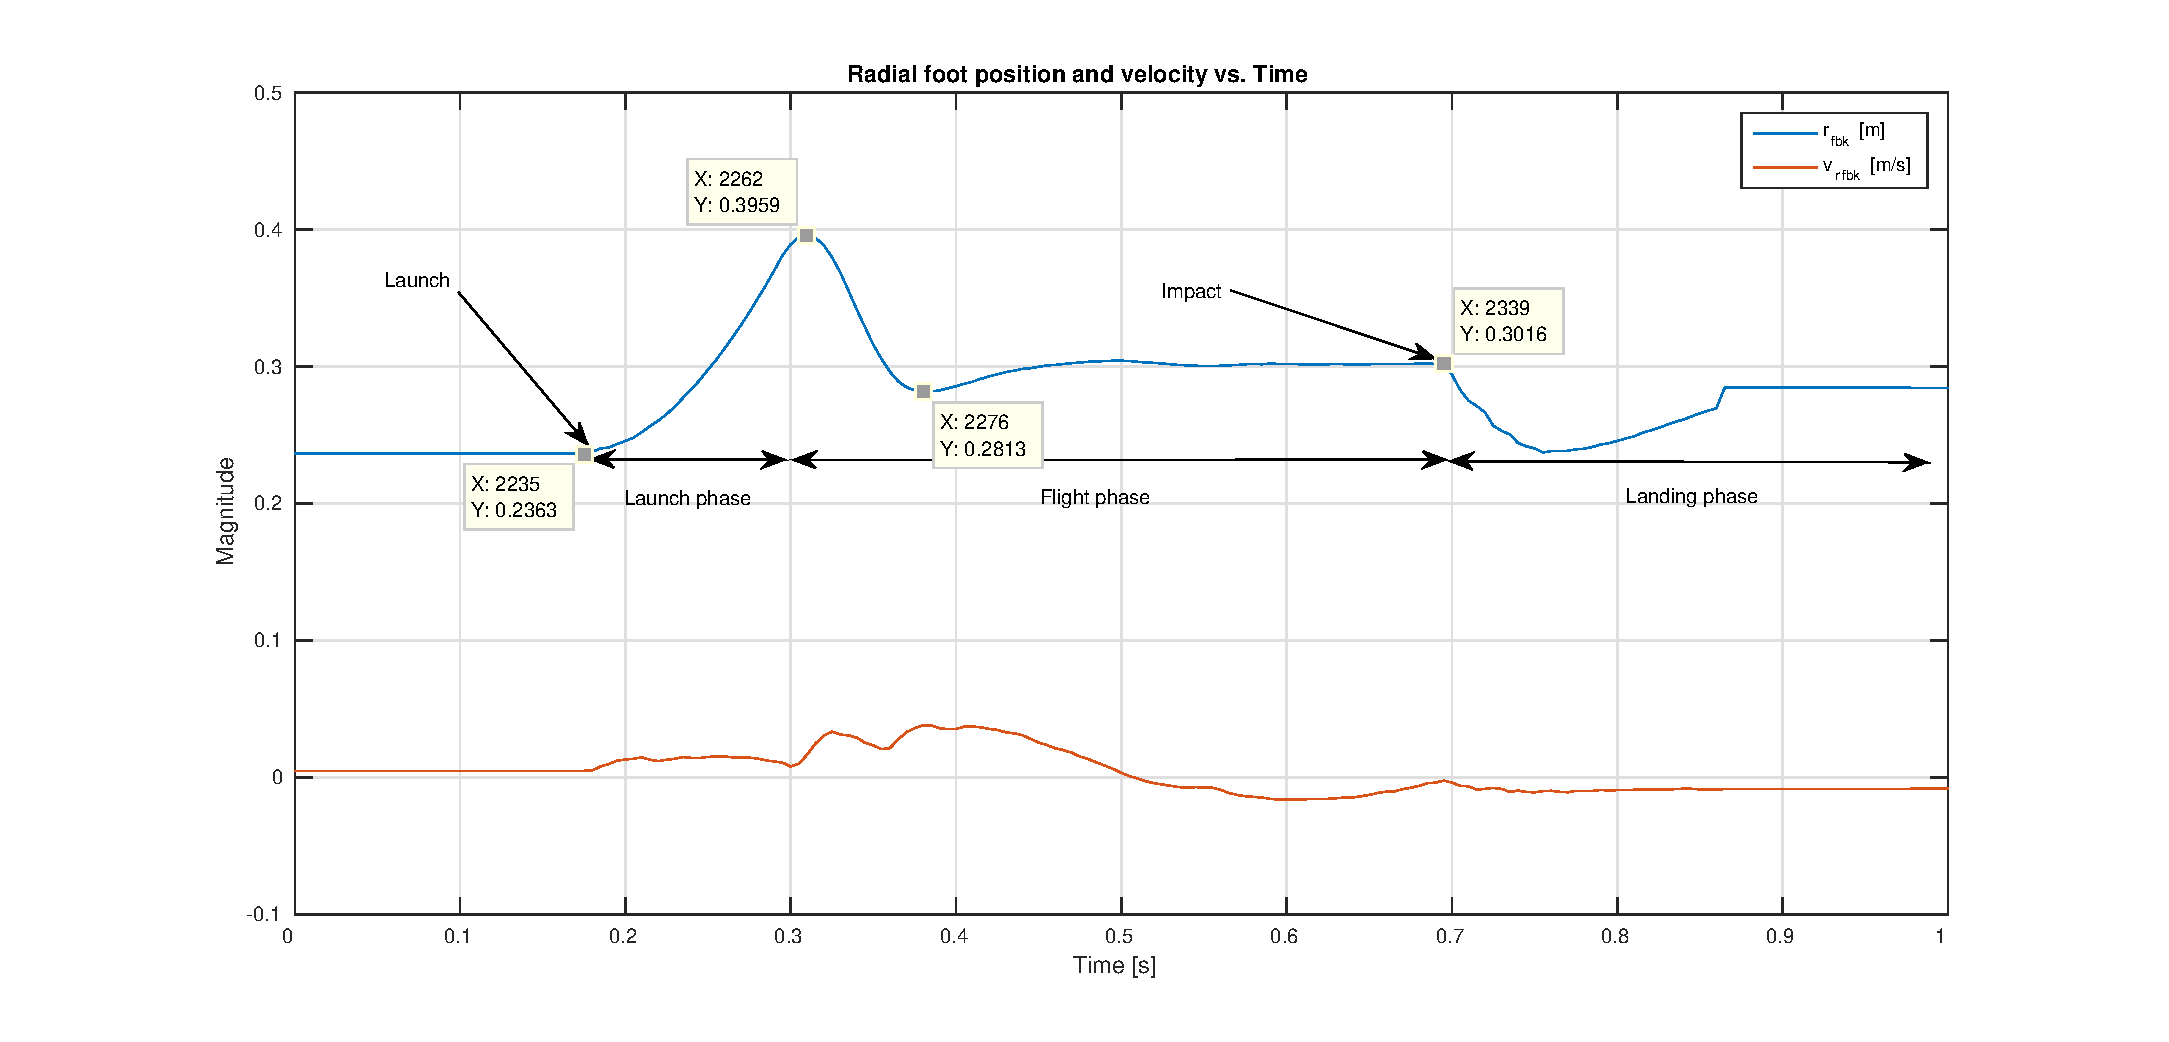
\includegraphics[width=1\textwidth]{images/experiments/jump/jump-foot-position-velocity.eps} 
\caption{Jump foot radial position and velocity (launch and compliant landing).}
\label{fig:Jump foot radial position and velocity}
\end{figure}

\begin{figure}
\centering
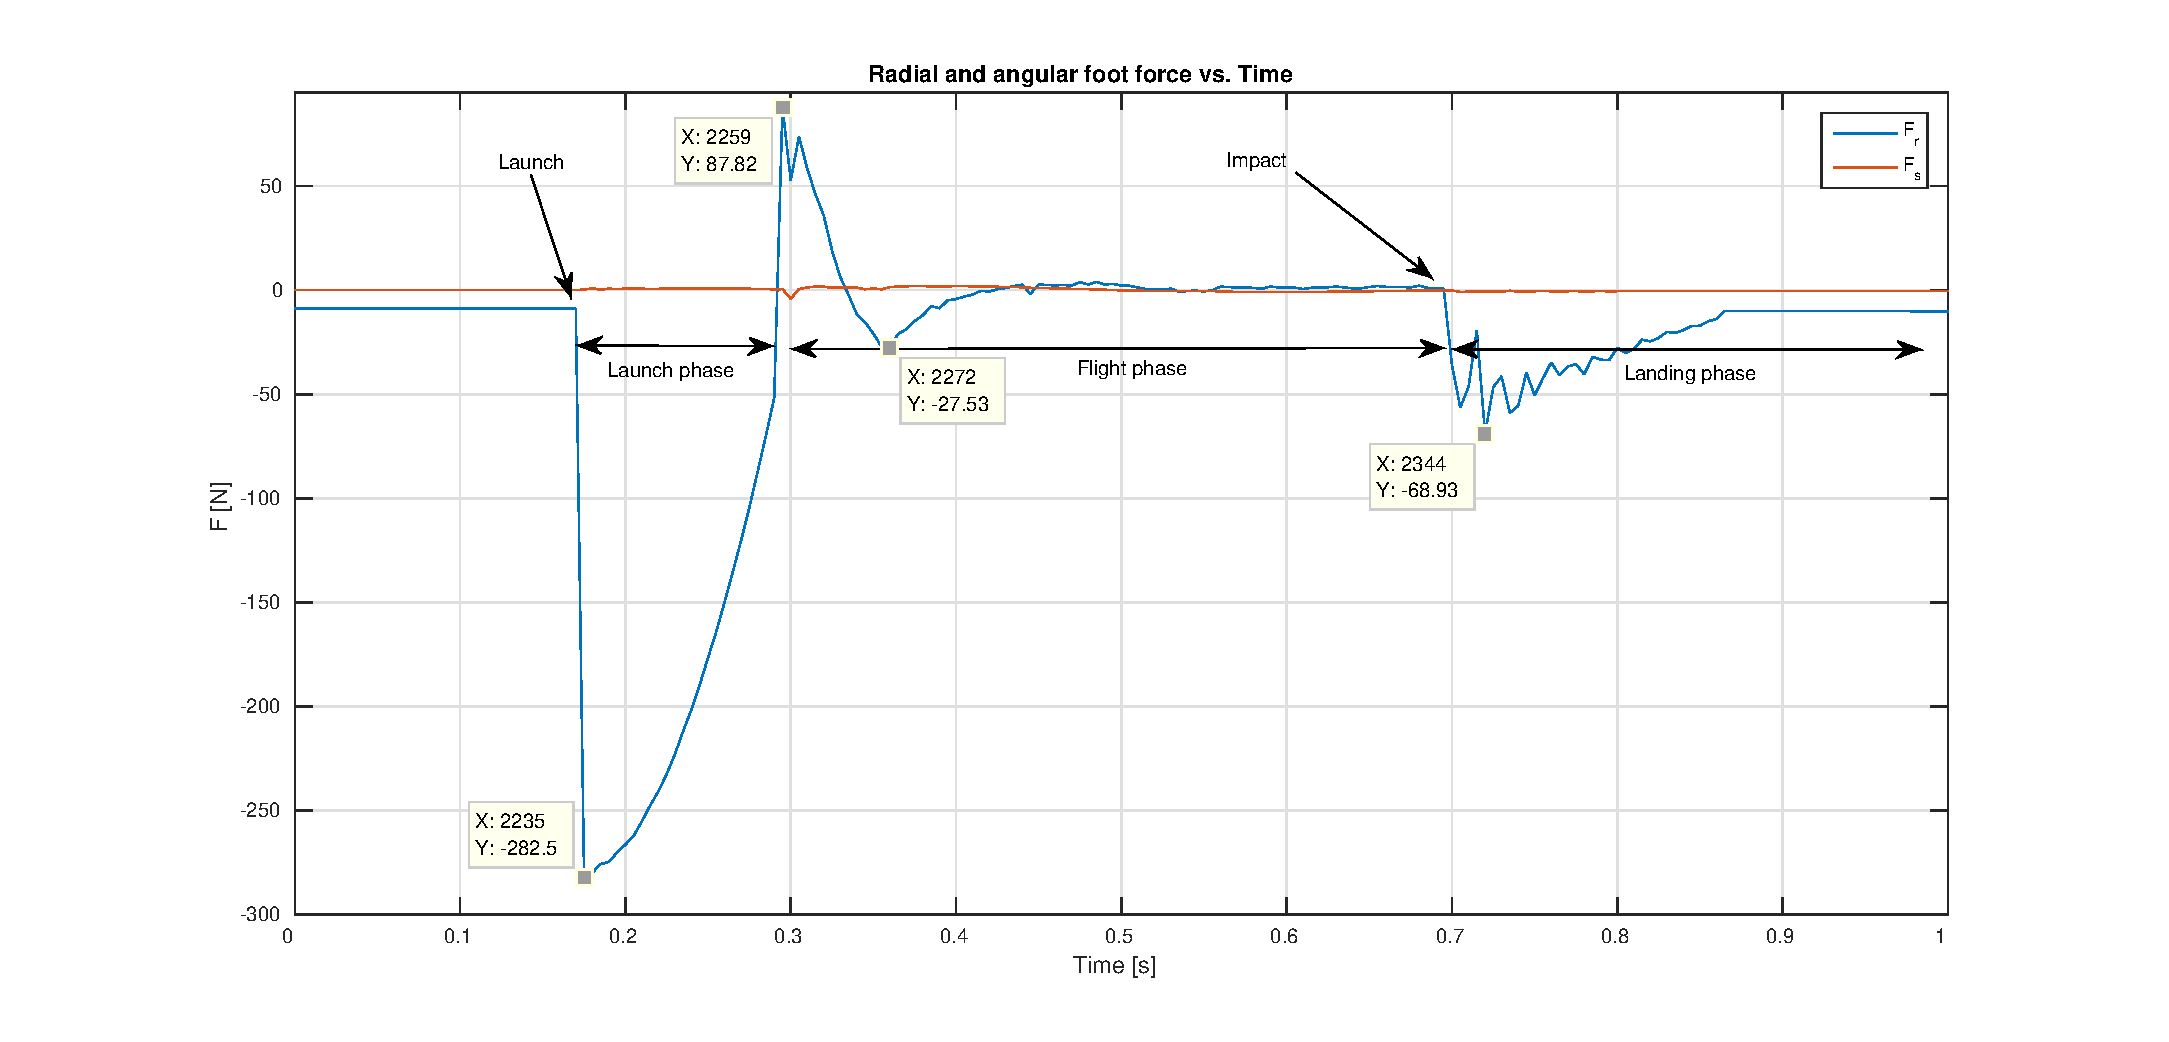
\includegraphics[width=1\textwidth]{images/experiments/jump/jump-foot-force.eps} 
\caption{Jump foot force output (launch and compliant landing).}
\label{fig:Jump foot force output}
\end{figure}

\begin{figure}
\centering
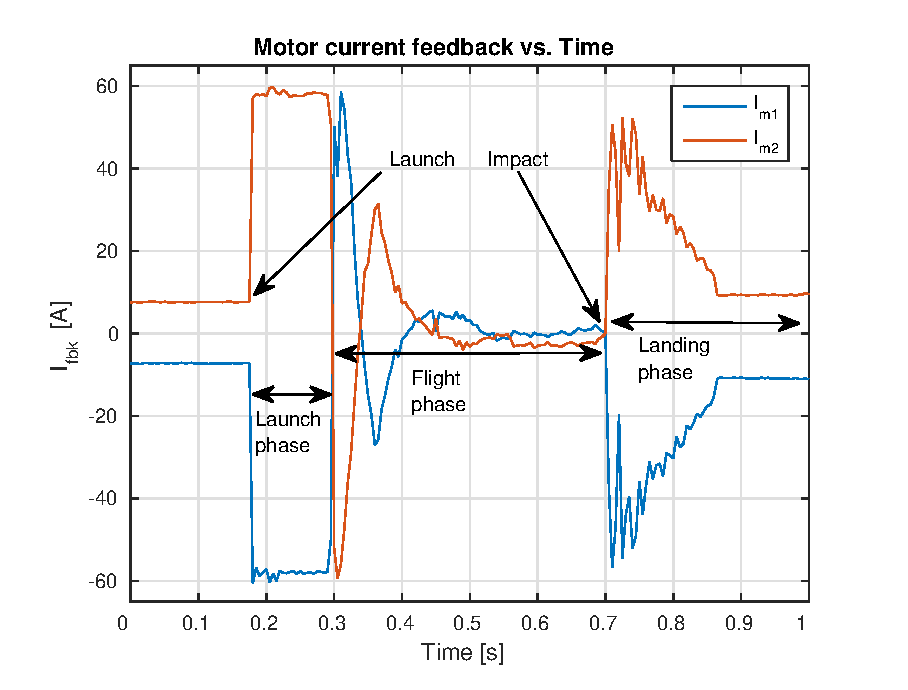
\includegraphics[width=1\textwidth]{images/experiments/jump/jump-current-feedback.eps} 
\caption{Jump motor current feedback (launch and compliant landing).}
\label{fig:jump-motor-current-feedback}
\end{figure}

\begin{figure}
\centering
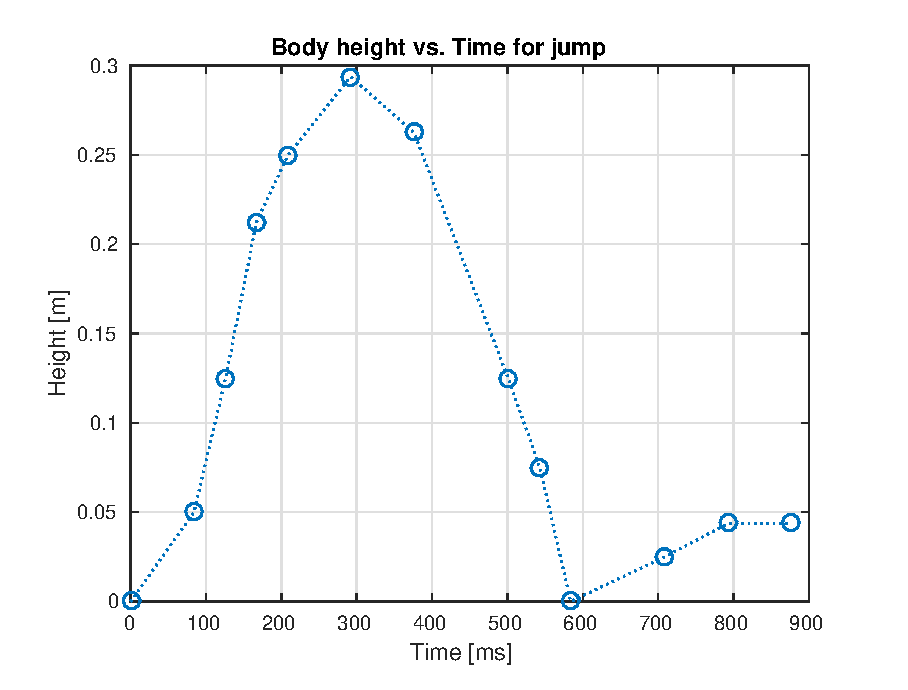
\includegraphics[width=1\textwidth]{images/experiments/jump/height-vs-time.eps} 
\caption{Height vs. time plot relative to body starting position.}
\label{fig:height-time-jump}
\end{figure}

\begin{figure}
\centering
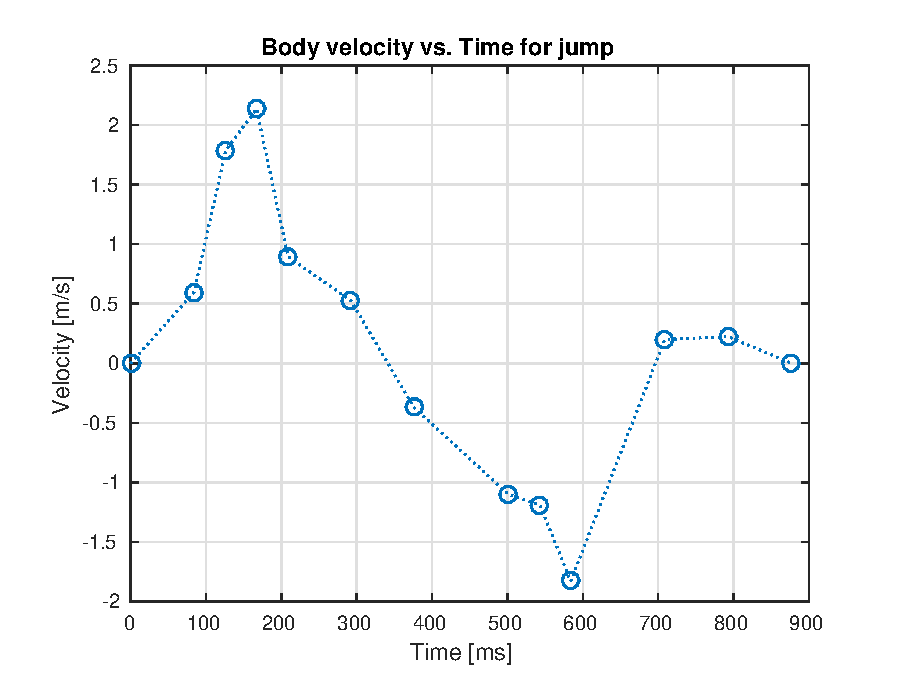
\includegraphics[width=1\textwidth]{images/experiments/jump/velocity-vs-time.eps} 
\caption{Velocity vs. time plot relative to body starting position.}
\label{fig:velocity-time-jump}
\end{figure}

\begin{figure}
\centering
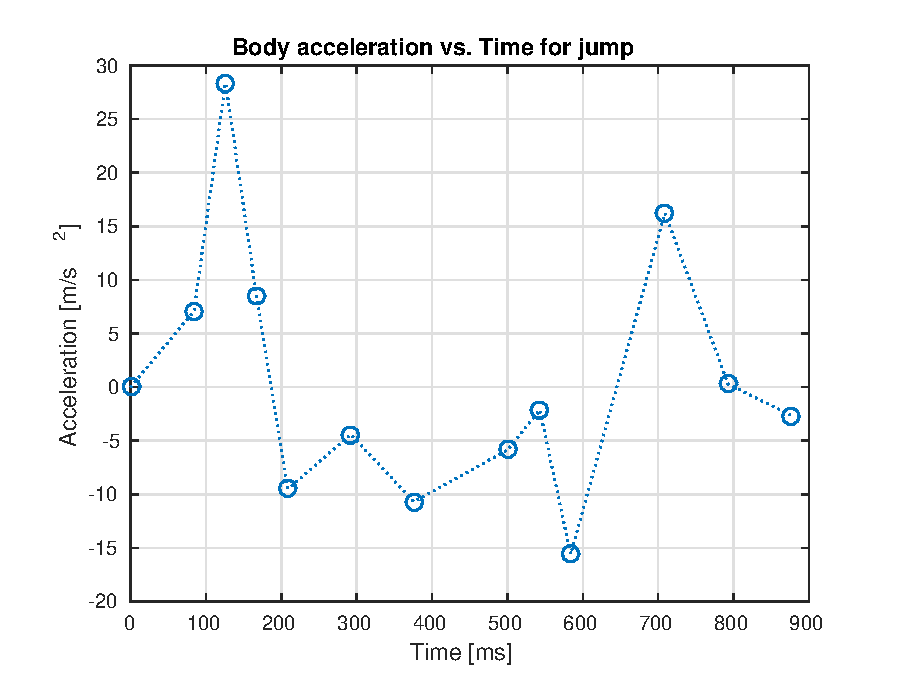
\includegraphics[width=1\textwidth]{images/experiments/jump/acceleration-vs-time.eps} 
\caption{Acceleration vs. time plot relative to body starting position.}
\label{fig:acc-time-jump}
\end{figure}

\begin{figure}
\centering
\subfloat[][Frame 0: Stance.]{
\includegraphics[width=0.3\textwidth]{images/experiments/jump/0.png} 
}
~
\subfloat[][Frame 1: Decompression.]{
\includegraphics[width=0.3\textwidth]{images/experiments/jump/1.png} 
}
~
\subfloat[][Frame 2: Decompression.]{
\includegraphics[width=0.3\textwidth]{images/experiments/jump/2.png} 
}

\subfloat[][Frame 3: Flight.]{
\includegraphics[width=0.3\textwidth]{images/experiments/jump/3.png} 
}
~
\subfloat[][Frame 4: Flight/recovery.]{
\includegraphics[width=0.3\textwidth]{images/experiments/jump/4.png} 
}
~
\subfloat[][Frame 5: Flight/recovery.]{
\includegraphics[width=0.3\textwidth]{images/experiments/jump/5.png} 
}
\caption{Jump: Stance and Flight Phase.}
\label{fig:Jump Stance and Flight Phase}
\end{figure}

\begin{figure}
\centering
\subfloat[][Frame 6: Freefall.]{
\includegraphics[width=0.3\textwidth]{images/experiments/jump/6.png} 
}
~
\subfloat[][Frame 7: Freefall.]{
\includegraphics[width=0.3\textwidth]{images/experiments/jump/7.png} 
}
~
\subfloat[][Frame 8: Impact.]{
\includegraphics[width=0.3\textwidth]{images/experiments/jump/8.png} 
}

\subfloat[][Frame 9: Compliant landing.]{
\includegraphics[width=0.3\textwidth]{images/experiments/jump/9.png} 
}
~
\subfloat[][Frame 10: Compliant landing.]{
\includegraphics[width=0.3\textwidth]{images/experiments/jump/10.png} 
}
~
\subfloat[][Frame 11: Compliant landing.]{
\includegraphics[width=0.3\textwidth]{images/experiments/jump/11.png} 
}
\caption{Jump: Freefall, Impact and Compliant Landing Phase.}
\label{fig:Jump Freefall, Impact and Compliant Landing Phase}
\end{figure}

\section{Current Tracking}

\subsection{Data Analysis}

\begin{figure}
\centering
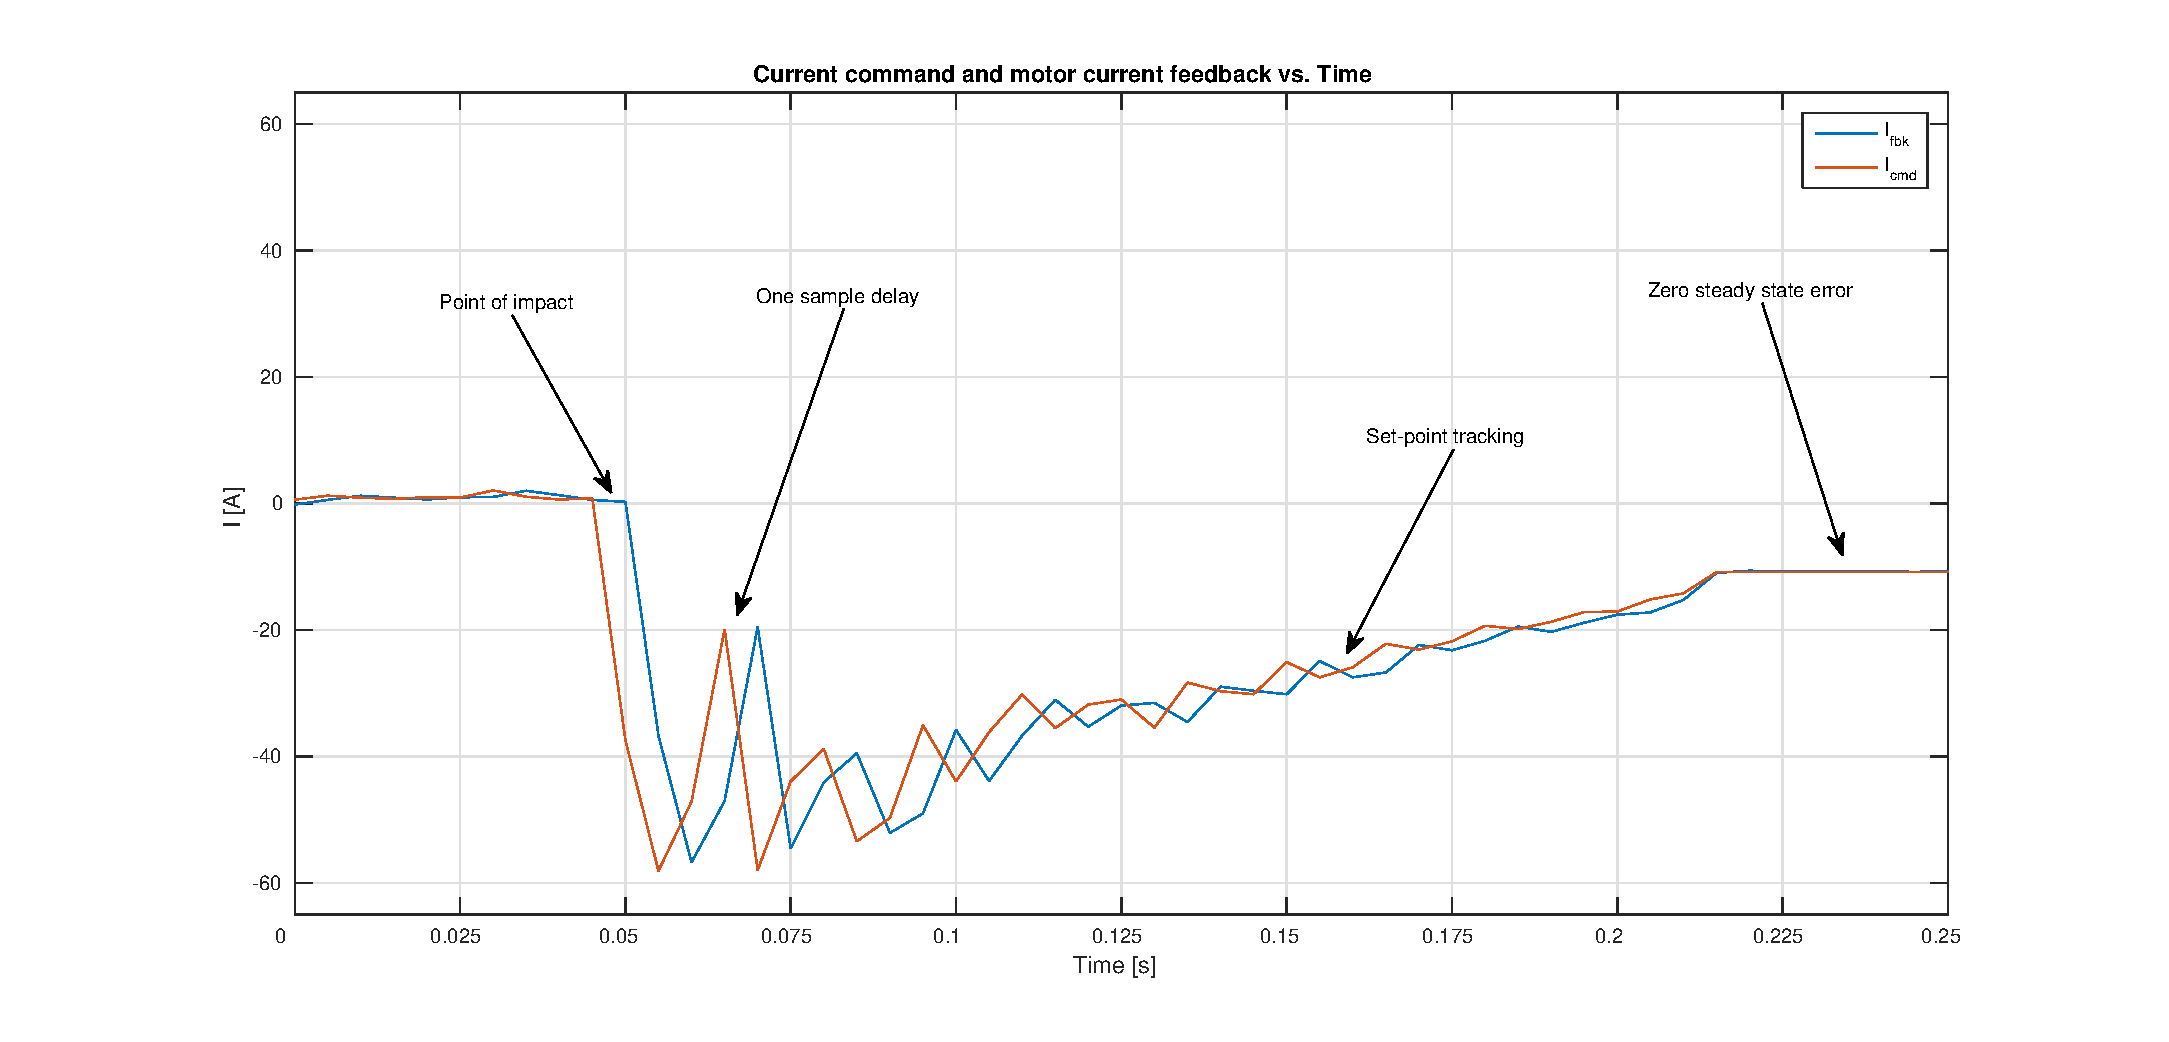
\includegraphics[width=1\textwidth]{images/experiments/current-tracking-impact.eps} 
\caption{Current control tracking.}
\label{fig:Current control tracking}
\end{figure}

\section{Force Estimation}
